\documentclass{standalone}
\usepackage{tikz}
\usetikzlibrary{patterns, positioning}
\usepackage[sfdefault]{ClearSans} %% option 'sfdefault' activates Clear Sans as the default text font
\usepackage[T1]{fontenc}

\begin{document}
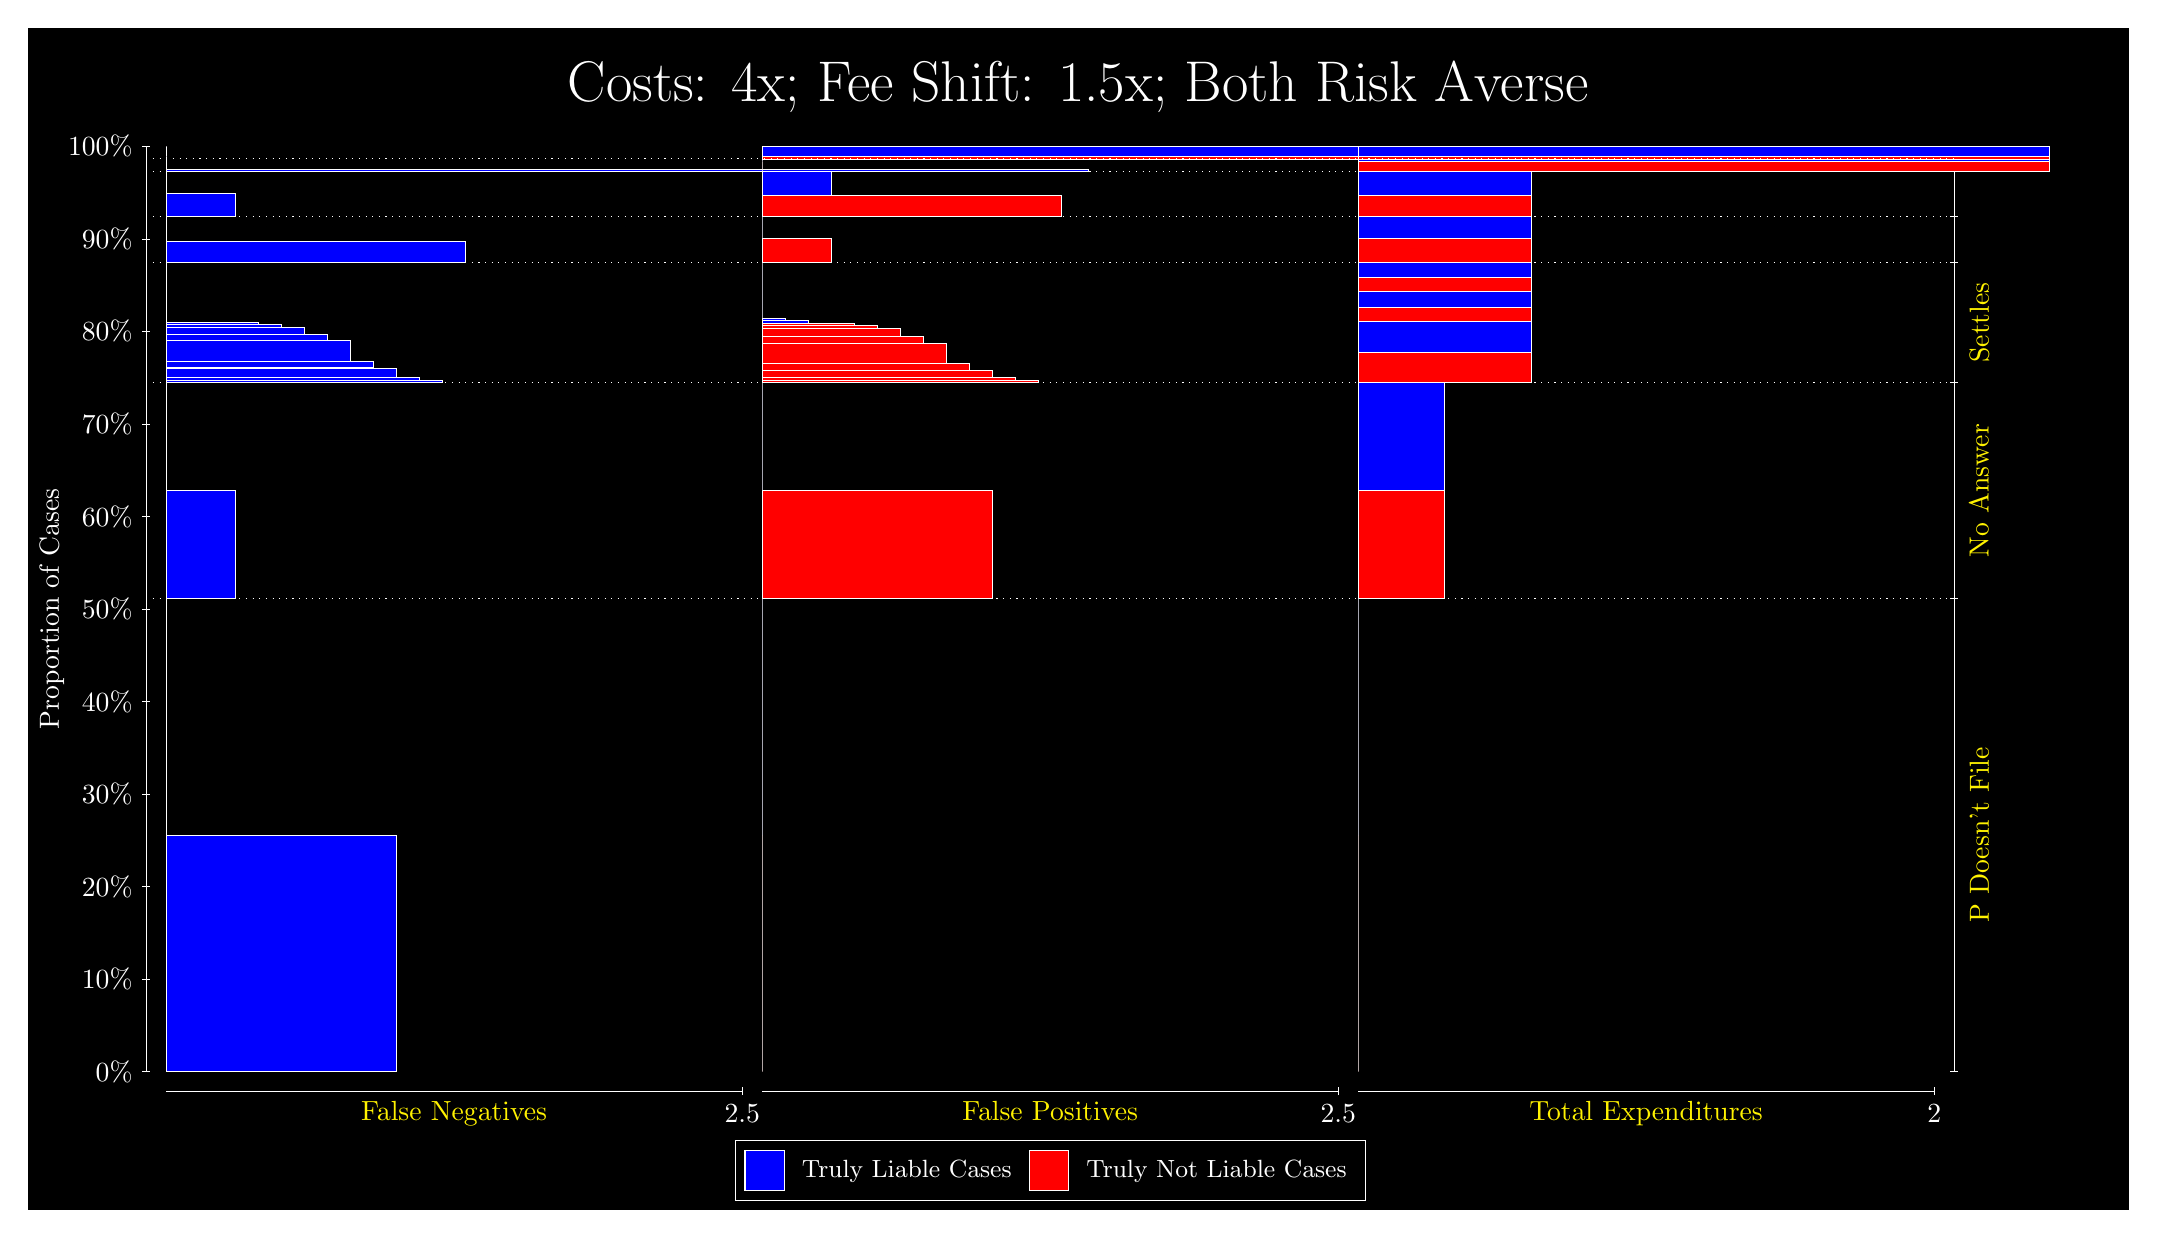
\begin{tikzpicture}
\draw[fill=black] (0,0) rectangle (26.667,15);
\draw[text=white] (0,13.5) rectangle (26.667,15) node[midway] {\huge Costs: 4x; Fee Shift: 1.5x; Both Risk Averse};
\draw[white, very thin] (1.5,1.75) -- (1.5,13.5);
\node[rotate=90, text=white, anchor=center] at (0.3, 7.625) {Proportion of Cases};
\draw[white, very thin] (1.45,1.75) -- (1.55,1.75);
\node[text=white, anchor=east] at (1.45, 1.75) {0\%};
\draw[white, very thin] (1.45,2.925) -- (1.55,2.925);
\node[text=white, anchor=east] at (1.45, 2.925) {10\%};
\draw[white, very thin] (1.45,4.1) -- (1.55,4.1);
\node[text=white, anchor=east] at (1.45, 4.1) {20\%};
\draw[white, very thin] (1.45,5.275) -- (1.55,5.275);
\node[text=white, anchor=east] at (1.45, 5.275) {30\%};
\draw[white, very thin] (1.45,6.45) -- (1.55,6.45);
\node[text=white, anchor=east] at (1.45, 6.45) {40\%};
\draw[white, very thin] (1.45,7.625) -- (1.55,7.625);
\node[text=white, anchor=east] at (1.45, 7.625) {50\%};
\draw[white, very thin] (1.45,8.8) -- (1.55,8.8);
\node[text=white, anchor=east] at (1.45, 8.8) {60\%};
\draw[white, very thin] (1.45,9.975) -- (1.55,9.975);
\node[text=white, anchor=east] at (1.45, 9.975) {70\%};
\draw[white, very thin] (1.45,11.15) -- (1.55,11.15);
\node[text=white, anchor=east] at (1.45, 11.15) {80\%};
\draw[white, very thin] (1.45,12.325) -- (1.55,12.325);
\node[text=white, anchor=east] at (1.45, 12.325) {90\%};
\draw[white, very thin] (1.45,13.5) -- (1.55,13.5);
\node[text=white, anchor=east] at (1.45, 13.5) {100\%};

\draw[white, very thin] (24.457,1.75) -- (24.457,13.5);
\draw[white, very thin] (24.407,1.75) -- (24.507,1.75);
\node[anchor=west] at (24.407, 1.75) {};
\draw[white, very thin] (24.407,7.7573) -- (24.507,7.7573);
\node[anchor=west] at (24.407, 7.7573) {};
\draw[white, very thin] (24.407,10.499) -- (24.507,10.499);
\node[anchor=west] at (24.407, 10.499) {};
\draw[white, very thin] (24.407,12.027) -- (24.507,12.027);
\node[anchor=west] at (24.407, 12.027) {};
\draw[white, very thin] (24.407,12.608) -- (24.507,12.608);
\node[anchor=west] at (24.407, 12.608) {};
\draw[white, very thin] (24.407,13.179) -- (24.507,13.179);
\node[anchor=west] at (24.407, 13.179) {};
\draw[white, very thin] (24.407,13.34) -- (24.507,13.34);
\node[anchor=west] at (24.407, 13.34) {};
\draw[white, very thin] (24.407,13.5) -- (24.507,13.5);
\node[anchor=west] at (24.407, 13.5) {};

\draw[white, very thin, fill=blue] (1.75,1.75) rectangle (4.6775,4.7536);
\draw[white, very thin, fill=red] (1.75,4.7536) rectangle (1.75,7.7573);
\draw[white, very thin, fill=blue] (1.75,7.7573) rectangle (2.6283,9.1281);
\draw[white, very thin, fill=red] (1.75,9.1281) rectangle (1.75,10.499);
\draw[white, very thin, fill=blue] (1.75,10.499) rectangle (5.2631,10.533);
\draw[white, very thin, fill=blue] (1.75,10.533) rectangle (4.9703,10.566);
\draw[white, very thin, fill=blue] (1.75,10.566) rectangle (4.6775,10.675);
\draw[white, very thin, fill=blue] (1.75,10.675) rectangle (4.3848,10.694);
\draw[white, very thin, fill=blue] (1.75,10.694) rectangle (4.3848,10.771);
\draw[white, very thin, fill=blue] (1.75,10.771) rectangle (4.092,11.042);
\draw[white, very thin, fill=blue] (1.75,11.042) rectangle (3.7993,11.119);
\draw[white, very thin, fill=blue] (1.75,11.119) rectangle (3.5065,11.207);
\draw[white, very thin, fill=blue] (1.75,11.207) rectangle (3.2138,11.236);
\draw[white, very thin, fill=blue] (1.75,11.236) rectangle (2.921,11.268);
\draw[white, very thin, fill=red] (1.75,11.268) rectangle (1.75,12.027);
\draw[white, very thin, fill=blue] (1.75,12.027) rectangle (5.5558,12.297);
\draw[white, very thin, fill=red] (1.75,12.297) rectangle (1.75,12.608);
\draw[white, very thin, fill=blue] (1.75,12.608) rectangle (2.6283,12.91);
\draw[white, very thin, fill=red] (1.75,12.91) rectangle (1.75,13.179);
\draw[white, very thin, fill=blue] (1.75,13.179) rectangle (13.46,13.211);
\draw[white, very thin, fill=red] (1.75,13.211) rectangle (1.75,13.34);
\draw[white, very thin, fill=red] (1.75,13.34) rectangle (1.75,13.372);
\draw[white, very thin, fill=blue] (1.75,13.372) rectangle (1.75,13.5);
\draw[white, very thin, fill=red] (9.3189,1.75) rectangle (9.3189,4.7537);
\draw[white, very thin, fill=blue] (9.3189,4.7537) rectangle (9.3189,7.7573);
\draw[white, very thin, fill=red] (9.3189,7.7573) rectangle (12.246,9.1281);
\draw[white, very thin, fill=blue] (9.3189,9.1281) rectangle (9.3189,10.499);
\draw[white, very thin, fill=red] (9.3189,10.499) rectangle (12.832,10.531);
\draw[white, very thin, fill=red] (9.3189,10.531) rectangle (12.539,10.562);
\draw[white, very thin, fill=red] (9.3189,10.562) rectangle (12.246,10.659);
\draw[white, very thin, fill=red] (9.3189,10.659) rectangle (11.954,10.746);
\draw[white, very thin, fill=red] (9.3189,10.746) rectangle (11.661,11.005);
\draw[white, very thin, fill=red] (9.3189,11.005) rectangle (11.368,11.09);
\draw[white, very thin, fill=red] (9.3189,11.09) rectangle (11.075,11.189);
\draw[white, very thin, fill=red] (9.3189,11.189) rectangle (10.783,11.222);
\draw[white, very thin, fill=red] (9.3189,11.222) rectangle (10.49,11.258);
\draw[white, very thin, fill=blue] (9.3189,11.258) rectangle (9.9044,11.29);
\draw[white, very thin, fill=blue] (9.3189,11.29) rectangle (9.6116,11.319);
\draw[white, very thin, fill=blue] (9.3189,11.319) rectangle (9.3189,12.027);
\draw[white, very thin, fill=red] (9.3189,12.027) rectangle (10.197,12.338);
\draw[white, very thin, fill=blue] (9.3189,12.338) rectangle (9.3189,12.608);
\draw[white, very thin, fill=red] (9.3189,12.608) rectangle (13.125,12.877);
\draw[white, very thin, fill=blue] (9.3189,12.877) rectangle (10.197,13.179);
\draw[white, very thin, fill=red] (9.3189,13.179) rectangle (9.3189,13.309);
\draw[white, very thin, fill=blue] (9.3189,13.309) rectangle (9.3189,13.34);
\draw[white, very thin, fill=red] (9.3189,13.34) rectangle (21.029,13.372);
\draw[white, very thin, fill=blue] (9.3189,13.372) rectangle (18.102,13.5);
\draw[white, very thin, fill=red] (16.888,1.75) rectangle (16.888,4.7537);
\draw[white, very thin, fill=blue] (16.888,4.7537) rectangle (16.888,7.7573);
\draw[white, very thin, fill=red] (16.888,7.7573) rectangle (17.986,9.1281);
\draw[white, very thin, fill=blue] (16.888,9.1281) rectangle (17.986,10.499);
\draw[white, very thin, fill=red] (16.888,10.499) rectangle (19.083,10.887);
\draw[white, very thin, fill=blue] (16.888,10.887) rectangle (19.083,11.274);
\draw[white, very thin, fill=red] (16.888,11.274) rectangle (19.083,11.461);
\draw[white, very thin, fill=blue] (16.888,11.461) rectangle (19.083,11.656);
\draw[white, very thin, fill=red] (16.888,11.656) rectangle (19.083,11.84);
\draw[white, very thin, fill=blue] (16.888,11.84) rectangle (19.083,12.027);
\draw[white, very thin, fill=red] (16.888,12.027) rectangle (19.083,12.338);
\draw[white, very thin, fill=blue] (16.888,12.338) rectangle (19.083,12.608);
\draw[white, very thin, fill=red] (16.888,12.608) rectangle (19.083,12.877);
\draw[white, very thin, fill=blue] (16.888,12.877) rectangle (19.083,13.179);
\draw[white, very thin, fill=red] (16.888,13.179) rectangle (25.67,13.309);
\draw[white, very thin, fill=blue] (16.888,13.309) rectangle (25.67,13.34);
\draw[white, very thin, fill=red] (16.888,13.34) rectangle (25.67,13.372);
\draw[white, very thin, fill=blue] (16.888,13.372) rectangle (25.67,13.5);
\draw[white, dotted] (1.5,7.7573) -- (24.457,7.7573);
\draw[white, dotted] (1.5,10.499) -- (24.457,10.499);
\draw[white, dotted] (1.5,12.027) -- (24.457,12.027);
\draw[white, dotted] (1.5,12.608) -- (24.457,12.608);
\draw[white, dotted] (1.5,13.179) -- (24.457,13.179);
\draw[white, dotted] (1.5,13.34) -- (24.457,13.34);
\draw[white, very thin] (1.75,1.5) -- (9.0689,1.5);
\node[text=yellow, anchor=north] at (5.4094, 1.5) {False Negatives};
\draw[white, very thin] (9.0689,1.45) -- (9.0689,1.55);
\node[text=white, anchor=north] at (9.0689, 1.45) {2.5};

\draw[white, very thin] (9.3189,1.5) -- (16.638,1.5);
\node[text=yellow, anchor=north] at (12.978, 1.5) {False Positives};
\draw[white, very thin] (16.638,1.45) -- (16.638,1.55);
\node[text=white, anchor=north] at (16.638, 1.45) {2.5};

\draw[white, very thin] (16.888,1.5) -- (24.207,1.5);
\node[text=yellow, anchor=north] at (20.547, 1.5) {Total Expenditures};
\draw[white, very thin] (24.207,1.45) -- (24.207,1.55);
\node[text=white, anchor=north] at (24.207, 1.45) {2};

\node[text=yellow, centered, rotate=90] at (24.777, 4.7537) {P Doesn't File};
\node[text=yellow, centered, rotate=90] at (24.777, 9.1281) {No Answer};
\node[text=yellow, centered, rotate=90] at (24.777, 11.263) {Settles};





\draw (12.978300999999998,1.5) node[draw=none] (baseCoordinate) {};
\begin{scope}[align=center]
        \matrix[scale=0.5, draw=white, below=0.5cm of baseCoordinate, nodes={draw}, column sep=0.1cm]{
            \node[rectangle, draw, minimum width=0.5cm, minimum height=0.5cm, fill=blue] {}; &
            \node[draw=none, font=\small, text=white] (B) {Truly Liable Cases}; &
            \node[rectangle, draw, minimum width=0.5cm, minimum height=0.5cm, fill=red] {}; &
            \node[draw=none, font=\small, text=white] (B) {Truly Not Liable Cases}; \\
            };
\end{scope}

\end{tikzpicture}
\end{document}